\subsection{Reconstruction metric}

The previous sections described a series of tensor 
approximations that exploit the redundancy of learnt convolutional 
layers. 
Approximation equations \ref{svdapprox}, \ref{eq:rankK}, \ref{blo2} minimize $L_2$ 
reconstruction error, which doesn't 
provide any guarantee that the network using approximated weights $\widetilde{W}$ 
will keep the same label prediction performance as the original network. 

One may ask  whether there exists a better criterion to guide the approximation than 
the $L_2$ norm. We propose here a simple modification of the metric of the form 
\begin{equation}
\label{poormansmaha}
\| W \|_\alpha^2 := \sum_p \alpha_p^2 W(p)^2 ~,
\end{equation}
where the sum runs over the tensor coordinates and $\alpha_p \geq 0$ are weights.
Since (\ref{poormansmaha}) is a reweighted Euclidiean metric, we can
still apply the previous approximation algorithms, by simply 
computing $W' = \alpha .* W$, where $.*$ denotes element-wise multiplication, 
then computing the approximation $\widetilde{W'}$ on $W'$ using the standard $L_2$ norm, 
and finally outputing $$\widetilde{W} = \alpha^{-1} .* \widetilde{W'}~.$$
The natural question is then how to choose the weights $\alpha_p$. For that purpose, 
we seek to emphasize coordinates more prone to produce prediction errors over 
coordinates whose effect is less harmful for the overall system. 

We can obtain such measurements as follows. Let $\Theta=\{W_1,\dots,W_S\}$ denote
the set of all parameters of the $S$-layer network, and let $U(I; \Theta)$ denote the output 
after the softmax layer of input image $I$.
We consider  a given input training set $(I_1,\dots,I_N)$ 
with known labels $(y_1,\dots,y_N)$. For each pair $(I_n, y_n)$, 
the compute the forward propagation pass $U(I_n, \Theta)$, and 
define as $\{\beta_n\}$ the indices of the $h$ largest values of  $U(I_n, \Theta)$ 
different from $y_n$.
Then, for a given layer $s$, we compute
\begin{equation}
\label{approxi}
d_{n,l,s} = \nabla_{W_s} \left( U(I_n, \Theta) - \delta(i - l)\right)~,~n\leq N\,,\, l \in \{\beta_n\}\,,\, s\leq S~,
\end{equation}
where $\delta(i-l)$ is the dirac distribution centered at $l$.
In other words, for each input we back-propagate the difference between the current prediction and the 
$h$ ``most dangerous" mistakes. 
The resulting weights $\alpha_p$ are then obtained by computing the average energy in the tensors $d_{n,l,s}$:
$$\alpha_p = \Big( \sum_{n,l} d_{n,l,s}(p)^2 \Big)^{1/2}~.$$

An even better metric can be obtained by considering the Mahalanobis distance defined from the covariance of 
$d$:
$$\| W \|_{maha}^2 = w \Sigma^{-1} w^T~,$$
where $w$ is the vector containing all the coordinates of $W$, and $\Sigma$ is the covariance of $(d_{n,l,s})_{n,l}$. 
However, we do not report results using this metric, since it requires inverting a matrix of size equal to the number 
of parameters, which can be prohibitively expensive in large networks.

Figure \ref{fig:components} compares the relationship between reconstruction error and prediction error 
using the unweighted and reweighted distance metrics, measured on
$4096$ samples of Imagenet for a range of different approximation hyperparameters.
 As expected, the reweighted $L_2$ distance correlates more strongly with
 performance loss. Consequently, optimizing the reweighted distance
 reduces the performance drop, for a given $\ell_2$ reconstruction error.

\begin{figure}[h]
\centering
\begin{minipage}{0.75\textwidth}
  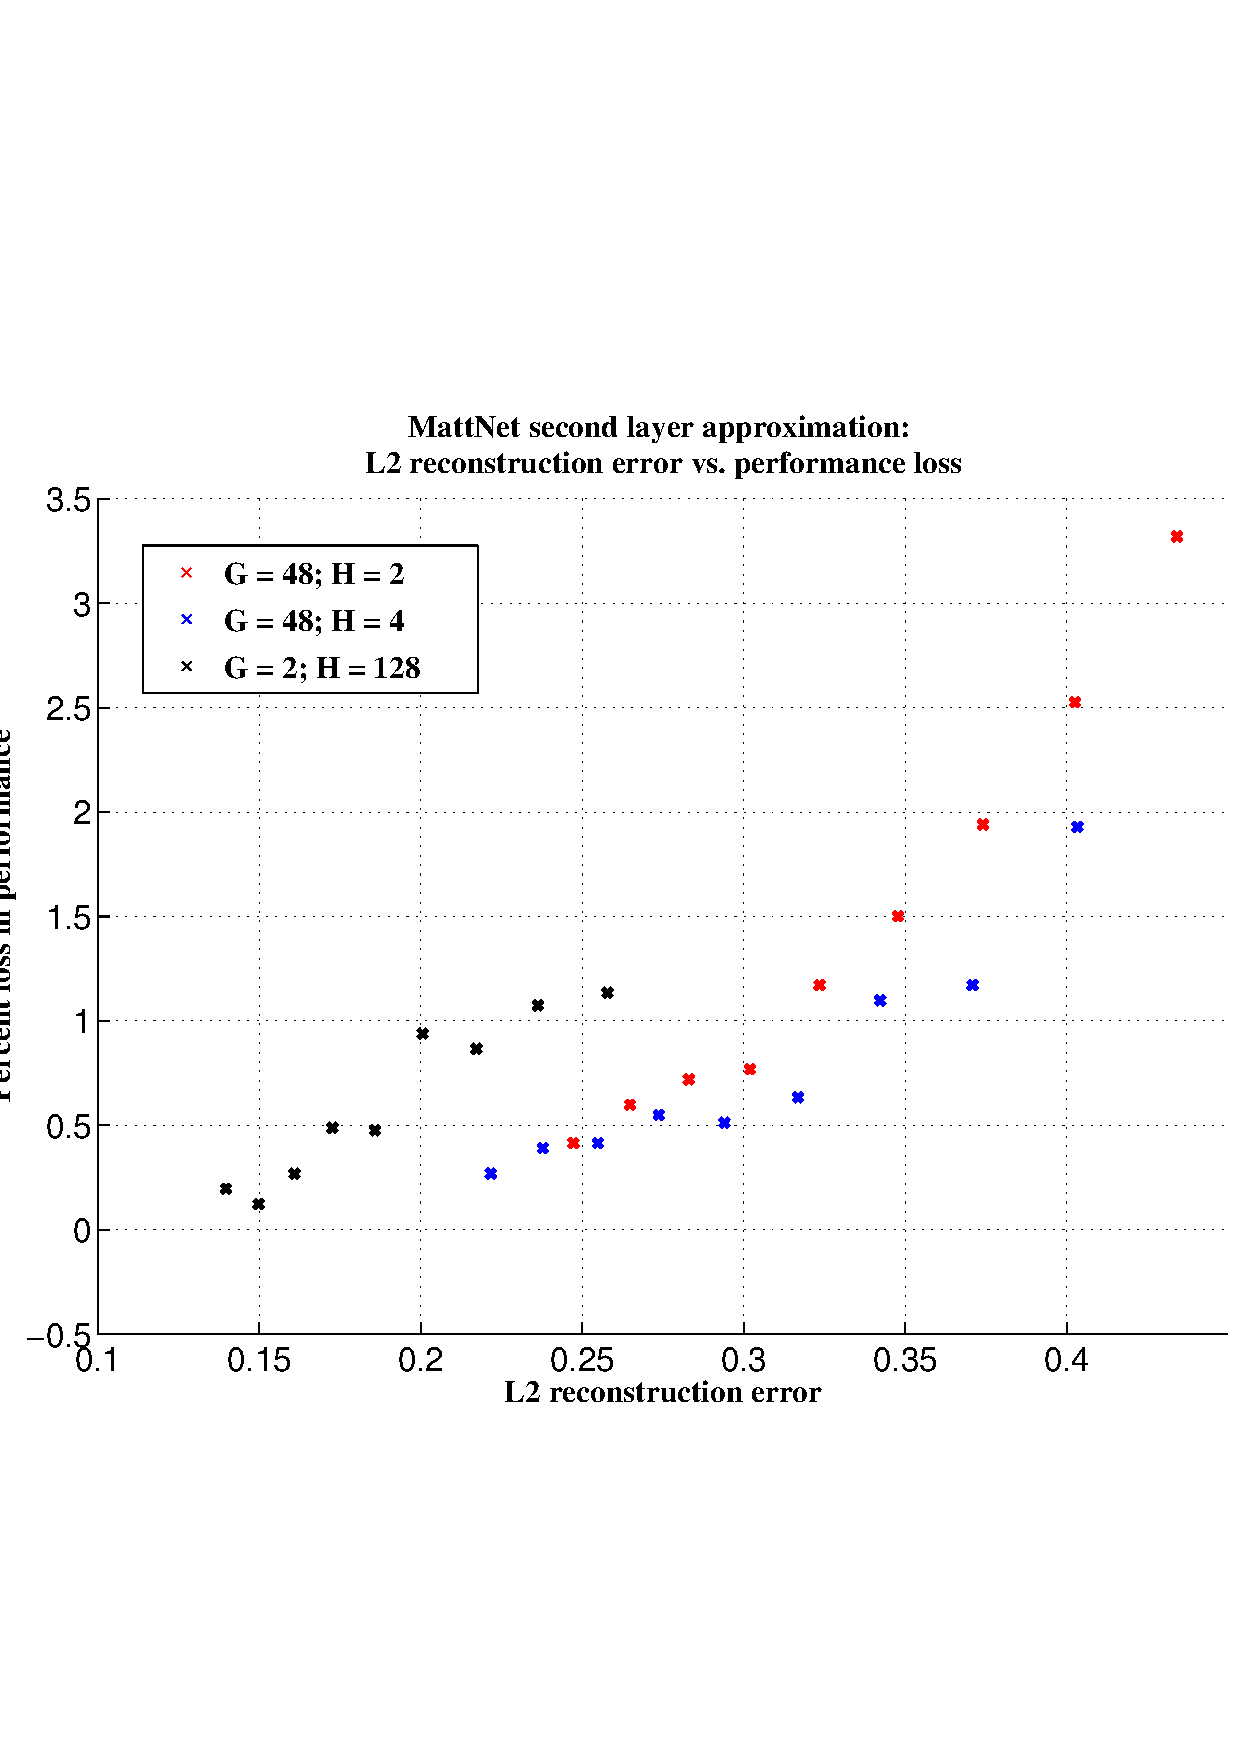
\includegraphics[width=0.5\linewidth]{img/biclustering_L2_vs_testerr_matt.pdf} 
\quad\quad
  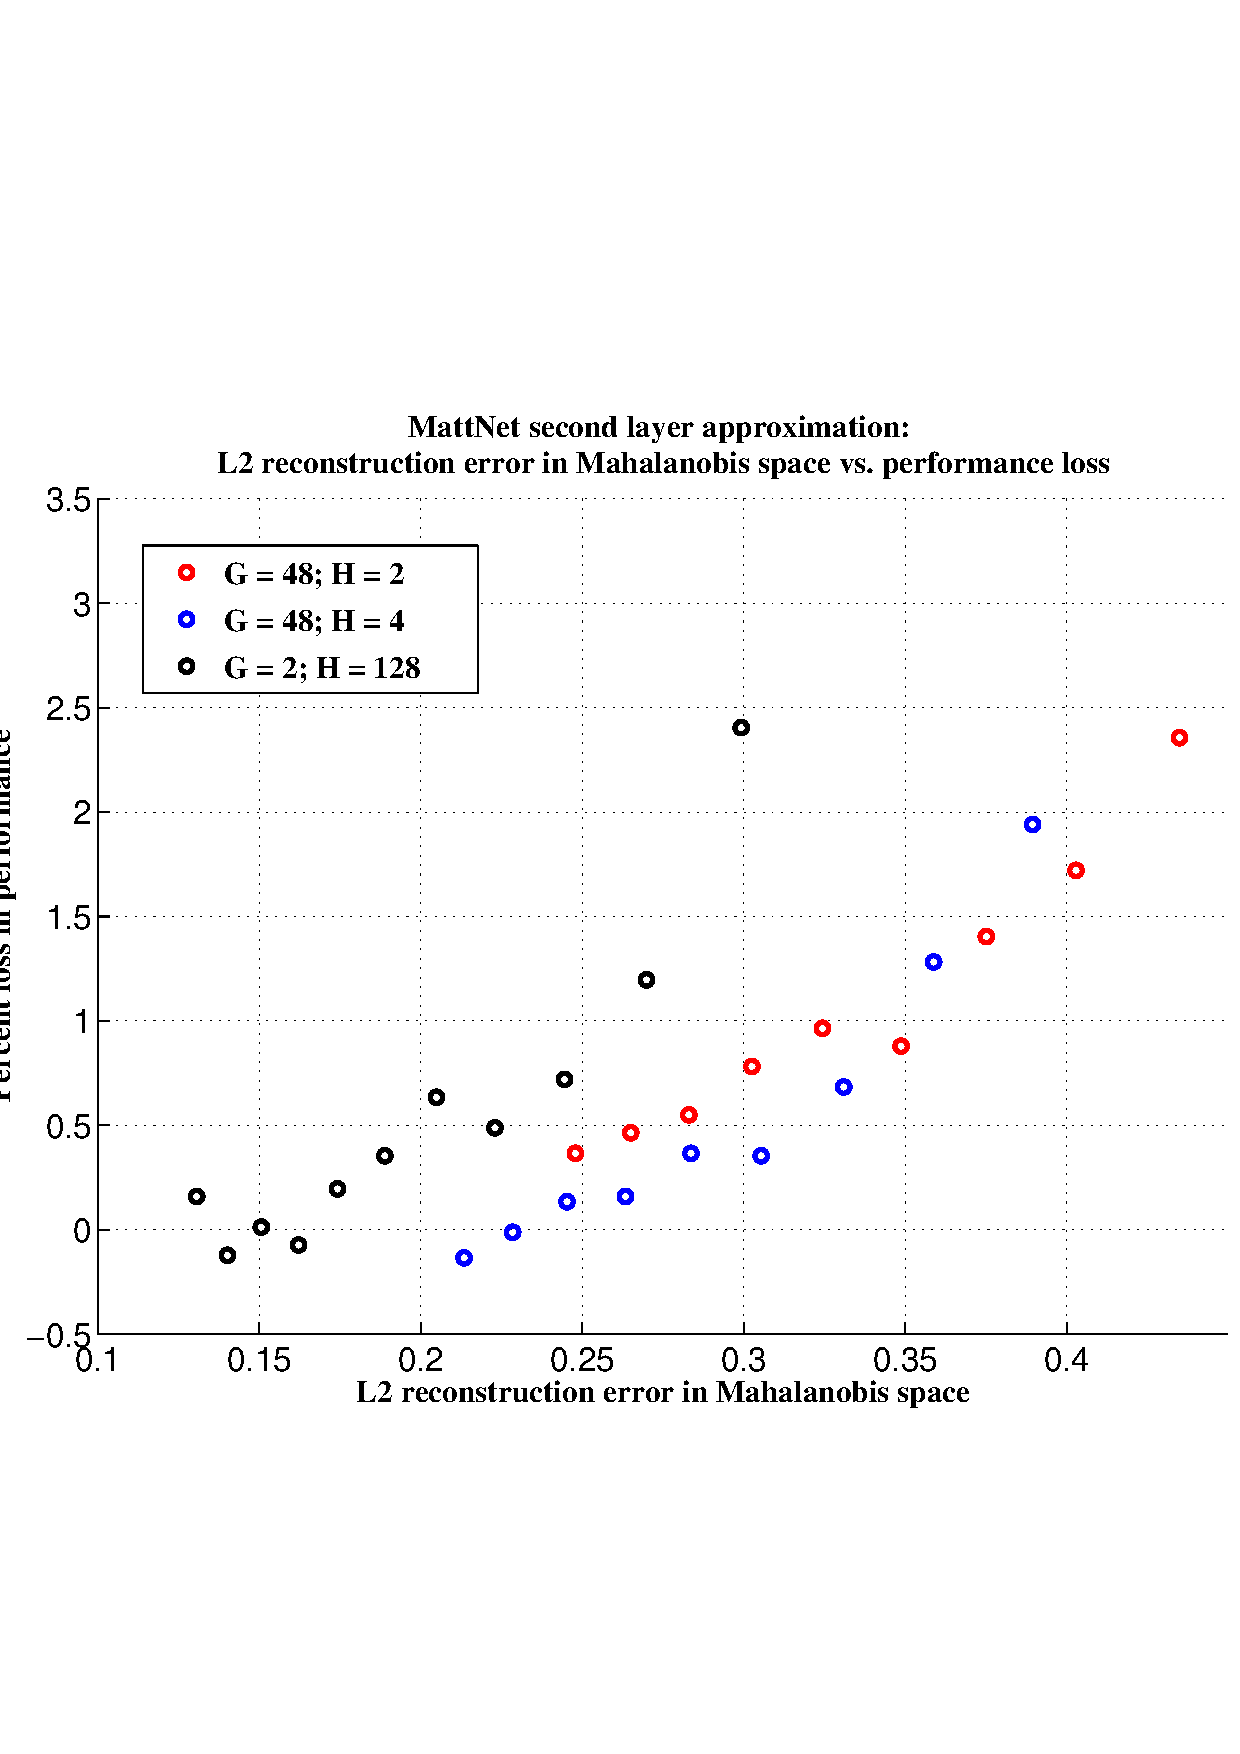
\includegraphics[width=0.5\linewidth]{img/biclustering_L2_vs_testerr_maha_matt.pdf} 
\end{minipage}
\vspace{-3mm}
\caption{$\ell_2$ reconstruction error of approximated weights in the
  original space (left) and the reweighted space (designed to match
  output error, see
  \ref{poormansmaha}) (right), versus decrease in peformance for a
  range of different approximation hyperparameters. Markers with the
  same color use the same settings for $G,H$ but vary the
  approximation rank. The reweighted space makes the correlation
  between $l_2$ and classification error more linear (e.g.~the red
  circles are well approximated by a line, but no so for the red
  crosses). Furthermore, for a given $l_2$ error, the performance loss
  is lower for the reweighted space. }
\label{fig:components}
\end{figure}

%Some ways of addressing it : 
%- Global approximation based on :
%	- backpropagation 
%	- Hessian
%- Local approximation : 
%	- relate to work of Simoncelli 

